% =============================================================================
% Standard journal paper (single file, ~12 pages with figures + references)
% Overleaf: paste as main.tex; create folder "figures" and upload from
% NEW WAY/docs/figures/: sece_phase3_architecture.png, benchmark_3h_heldout.png,
% tsne_era5_63d.png, case_study_laila_trajectories.png
% =============================================================================
\documentclass[11pt]{article}
\usepackage[margin=1in]{geometry}
\usepackage{graphicx}
\graphicspath{{figures/}}
\usepackage{booktabs}
\usepackage{multirow}
\usepackage{amsmath}
\usepackage{hyperref}
\usepackage{cite}

\newcommand{\sece}{SECE}
\newcommand{\secefull}{Subset-Expert Context-Aware Ensemble (\sece{} v2 Phase~3)}
\newcommand{\bob}{Bay of Bengal}
\newcommand{\era}{ERA5}
\newcommand{\ibtracs}{IBTrACS}
\newcommand{\km}{\,km}
\newcommand{\bonf}{0.0071}

\title{ERA5-Augmented Ensemble Learning for Multi-Horizon Tropical Cyclone Track Prediction over the Bay of Bengal: A Leakage-Aware Benchmark}

\author{[Author One]\thanks{Corresponding author: [email]} \and [Author Two]\\
\textit{[Affiliation, Department, City, Country]}}

\date{}

\begin{document}
\maketitle

\begin{abstract}
Accurate short-to-medium-range cyclone track forecasting supports disaster preparedness over the \bob{}, one of the world's most cyclone-exposed basins.
We benchmark eight track-prediction systems---\secefull{} and seven baselines---at 3, 12, 24, and 48-hour lead times on North Indian Ocean \ibtracs{} storms (genesis 1940--2024).
After quality control, 852 storms and 27{,}728 three-hourly origins define the modeling table; 583 storms (15{,}605 samples) support multi-horizon targets.
Forty-nine track/physics inputs are augmented with 14 \era{} point reanalysis features (winds at 850/500/200\,hPa, mean sea level pressure, SST, steering flow, vertical shear).
We identify and correct a subtle test-set leakage mode in which cross-run architecture decisions were guided by repeated inspection of test performance, and adopt a strict development versus held-out seed protocol (nine seeds each; held-out evaluated once).
On pooled held-out tests (442 unique storm IDs), \sece{} significantly outperforms all seven baselines at 3 and 12\,h (paired Wilcoxon on per-storm medians, Bonferroni correction, $p<\bonf$).
At 24 and 48\,h, \sece{} is statistically indistinguishable from the strongest tree ensembles while remaining significantly better than CatBoost and, at 24\,h, CB+MotionNN.
Controlled ablations show that a dedicated atmospheric ``environ'' expert adds value over track-only features; spatial-patch \era{} features were tested and not adopted.
CNN-GRU and BLSTM were not re-evaluated on the locked held-out confirm.
\end{abstract}

\section{Introduction}
\label{sec:intro}

Operational numerical weather prediction (NWP) remains the reference for cyclone track guidance, but data-driven models trained on historical best tracks offer a lightweight complement where compute or assimilation capacity is limited \cite{demaria2013,goerss2000}.
For the \bob{} rim---including Bangladesh, one of the most cyclone-vulnerable coasts---reliable 3--48\,h track guidance feeds evacuation timing, port closures, and surge planning \cite{paul2010,mohapatra2015,emanuel2005}.

Despite growing interest in machine learning for tropical cyclones, three gaps persist for the North Indian Ocean: (i)~narrow architectural benchmarking; (ii)~inconsistent multi-horizon evaluation; (iii)~unclear incremental value of atmospheric reanalysis beyond kinematics \cite{prat2021,chan2005,liu2020}.
A fourth methodological gap is equally important: ensemble studies often iterate design while inspecting test-set rank tables, inflating apparent generalization unless confirm data are firewalled \cite{cawley2010,gneiting2014}.

\textbf{Contributions.}
\begin{itemize}
\item An eight-system, four-horizon benchmark under storm-wise splits with bootstrap CIs and pooled significance testing (442 unique test storm IDs across nine held-out seeds).
\item \secefull{}, combining subset-specific tree experts, a dedicated \era{} environ channel, champion baselines, and validation-only fusion routing (Phase~3).
\item Controlled ablations (track-only, point \era{}, environ expert, 5$^\circ$/3$^\circ$ spatial patches) with transparent negative results.
\item A reproducible artifact trail aligned with the locked ``NEW WAY'' pipeline (datasets, held-out predictions, writeup tables).
\end{itemize}

\section{Related work}
Statistical-dynamical aids and climatological--persistence baselines remain operational references \cite{neumann1972,kaplan2003,sampson2018}.
Machine-learning track models include tree ensembles and deep sequence architectures \cite{wu2018,chen2020,lee2021}; on tabular, engineered storm--environment data, trees often match or exceed deep networks at comparable sample sizes \cite{grinsztajn2022,probst2019}.
\era{} and satellite-era reanalysis provide gridded environmental context at storm locations \cite{hersbach2020,velden2006,barnes2013,reichstein2019}.
Basin-specific BoB studies have emphasized intensity or single-lead track tasks more than multi-horizon, leakage-controlled ensemble benchmarks \cite{chan2005,walsh2015}.

\section{Data and experimental design}
\label{sec:data}

\subsection{Sources and domain}
Storm tracks come from \ibtracs{} v4 (North Indian Ocean) \cite{knapp2010,schreck2014}.
\era{} reanalysis \cite{hersbach2020} on 30--5$^\circ$N, 70--102$^\circ$E is joined at each 3-hourly track time ($\approx$10.5\,GB source NetCDF over 551 storm-months).

\subsection{Quality control and counts}
Genesis-year filtering 1940--2024 yields 852 storms and 27{,}728 QC 3-hourly rows.
Multi-horizon labels require sufficient forward track length; 583 storms contribute 15{,}605 multi-horizon origins (12, 24, 48\,h).
Storm-wise 70:15:15 train/validation/test splits are redrawn per seed ($\approx$408/87/88 storms per held-out seed).
Significance analysis pools test predictions across nine held-out seeds $[0,1,2,7,13,99,123,2024,2026]$; 442 is the count of distinct storm IDs in that pooled test set.

\subsection{Features}
\textbf{Track/physics (49):} position lags, motion kinematics, seasonality, recurvature proxies, land interaction, and missingness flags \cite{holland1983}.
\textbf{\era{} point (14):} 850/500/200\,hPa winds, MSLP, SST (with coastal imputation flag; $\approx$38\% of rows), steering ($u,v$), shear ($u,v$, magnitude).
Spatial 5$^\circ$/3$^\circ$ patch statistics were extracted for ablation but not locked.

\subsection{Date window}
Fixed-test comparison of genesis windows 1940--2024, 1979--2024, and 1990--2024 supported retaining 1940--2024: long-lead advantage persisted on a common modern test draw while short-lead gaps were largely compositional \cite{kossin2013,walsh2015}.

\section{Test-set leakage and validation protocol}
\label{sec:leakage}

Early development advanced architectural phases using test-set rank inspection across a single split.
Base learners were fit without test labels, but the \emph{architecture} was tuned with test feedback---a common but under-reported leakage mode \cite{cawley2010}.
We separated nine \emph{development} seeds $[3,4,5,6,8,9,10,11,14]$ (architecture lock only) from nine \emph{held-out} seeds evaluated once after freeze.
Development and held-out mean medians align closely (e.g., 48\,h \sece{} $\approx$247\,\km{} in both tiers), supporting that Phase~3 was not overfit to a single confirm split.

Primary metric: median great-circle (Haversine) error in kilometers.
Held-out confirm adds 10{,}000 storm-bootstrap 95\% CIs and paired Wilcoxon tests versus \sece{} with Bonferroni threshold $\alpha/7 \approx \bonf$.

\section{Methods}
\label{sec:methods}

\subsection{Baselines}
Seven comparators: Stacking Ensemble (RF+XGB+LGB with Ridge meta), Persistence Residual Cascade (PRC), Random Forest, LightGBM, XGBoost, CatBoost, and CB+MotionNN (CatBoost + 64-32-16 MLP on motion residuals).
Uniform tree hyperparameters (300 estimators, depth 6, learning rate 0.01) isolate architectural differences.

\subsection{\sece{} Phase~3}
Horizon-specific subsets (3\,h: position, motion, environ, full; 12--48\,h: motion, physics, environ, full) each train four tree algorithms, fused by NNLS per subset.
Subset-NNLS signals join seven champions in horizon-specific fusion candidates (degree-NNLS, km-NNLS, stacking-residual at 3\,h).
A validation-best router selects the lowest validation median-\km{} candidate per seed; test predictions use the frozen choice without test peeking (Fig.~\ref{fig:arch}).

\subsection{Training details}
Table~\ref{tab:hyp} summarizes locked hyperparameters (uniform across tree baselines unless noted).
LightGBM uses 63 leaves; XGBoost subsample/colsample 0.8; Stacking Ridge meta-learner trained on 150 CV meta-predictions.

\begin{table}[ht]
\caption{Locked tree and meta-learner hyperparameters.}
\label{tab:hyp}
\centering
\small
\begin{tabular}{@{}ll@{}}
\toprule
Component & Setting \\
\midrule
Tree estimators & 300 \\
Max depth & 6 (CatBoost: depth 6) \\
Learning rate & 0.01 \\
LightGBM num\_leaves & 63 \\
XGBoost subsample / colsample & 0.8 / 0.8 \\
Stacking Ridge meta & 150 CV meta-samples \\
MotionNN (CB+MotionNN) & 64-32-16, lr 0.01, max 100 iter \\
\bottomrule
\end{tabular}
\end{table}

\subsection{Systems not in held-out table}
CNN-GRU and BLSTM were explored in development but were \textbf{not} re-trained in the locked held-out run; they must not be cited on the confirm table.

\section{Results}
\label{sec:results}

\subsection{Development ablations}
Table~\ref{tab:abl} reports \sece{} rank-1 frequency (seeds with lowest test median among eight systems) and mean median \km{} across development seeds.
Point \era{} reduced 48\,h mean error from 250.26 to 246.80\,\km{} (8/9 seeds improved).
The environ expert improved 24\,h mean to 99.43\,\km{} (best balance among tested configs).
Spatial patches increased 3--12\,h rank-1 frequency but did not justify complexity at 24--48\,h (negative result).

\begin{table}[ht]
\caption{Development-seed ablation: \sece{} rank-1 count / mean median \km{} (nine dev seeds).}
\label{tab:abl}
\centering
\small
\begin{tabular}{@{}lcccc@{}}
\toprule
Configuration & 3\,h & 12\,h & 24\,h & 48\,h \\
\midrule
Track-only (no \era{}) & 5/9·4.84 & 3/9·35.48 & 3/9·100.48 & 0/9·250.26 \\
+ Point \era{} & 5/9·4.93 & 7/9·35.59 & 2/9·99.86 & 1/9·246.80 \\
+ Environ expert (locked) & 5/9·4.93 & 6/9·35.56 & 3/9·99.43 & 2/9·246.94 \\
+ Spatial 5$^\circ$ & 7/9·4.93 & 7/9·35.56 & 1/9·99.74 & 1/9·246.55 \\
+ Spatial 3$^\circ$ & 7/9·4.93 & 7/9·35.66 & 2/9·99.42 & 3/9·247.00 \\
Held-out (locked environ) & 6/9·4.90 & 6/9·35.63 & 2/9·101.21 & 1/9·246.99 \\
\bottomrule
\end{tabular}
\end{table}

\subsection{Held-out confirm}
Table~\ref{tab:heldout} lists pooled medians and CIs for all eight evaluated systems (34{,}114 test samples at 3\,h; 21{,}442 at 12--48\,h).
At 3 and 12\,h, \sece{} beats every baseline with Bonferroni significance (Table~\ref{tab:wilcox}).
At 24\,h, differences versus Stacking, PRC, LightGBM, and XGBoost are not significant after correction; \sece{} remains significantly better than CatBoost and CB+MotionNN.
At 48\,h, \sece{} ties leading ensembles within CI overlap; only CatBoost is significantly worse.
\sece{} is never significantly \emph{worse} than any baseline at any horizon.

\begin{table*}[t]
\caption{Held-out test performance: median great-circle error (\km{}) with 95\% bootstrap CI. Nine held-out seeds pooled; 442 distinct storm IDs.}
\label{tab:heldout}
\centering
\small
\begin{tabular}{@{}llrrr@{}}
\toprule
Horizon & System & Median & 95\% CI low & 95\% CI high \\
\midrule
\multirow{8}{*}{3\,h}
  & \textbf{\sece{} v2 Phase~3} & \textbf{4.895} & 4.714 & 5.079 \\
  & Random Forest & 4.927 & 4.734 & 5.125 \\
  & Stacking Ensemble & 4.945 & 4.763 & 5.123 \\
  & CB+MotionNN & 5.813 & 5.701 & 5.928 \\
  & LightGBM & 6.026 & 5.889 & 6.168 \\
  & XGBoost & 6.411 & 6.243 & 6.580 \\
  & CatBoost & 8.479 & 8.284 & 8.691 \\
  & PRC & 8.872 & 8.707 & 9.058 \\
\midrule
\multirow{8}{*}{12\,h}
  & \textbf{\sece{} v2 Phase~3} & \textbf{35.538} & 34.208 & 36.925 \\
  & Stacking Ensemble & 36.146 & 34.744 & 37.701 \\
  & Random Forest & 36.901 & 35.525 & 38.323 \\
  & LightGBM & 36.928 & 35.498 & 38.338 \\
  & XGBoost & 36.947 & 35.531 & 38.416 \\
  & PRC & 37.177 & 35.704 & 38.527 \\
  & CB+MotionNN & 37.413 & 36.047 & 38.949 \\
  & CatBoost & 42.028 & 40.381 & 43.656 \\
\midrule
\multirow{8}{*}{24\,h}
  & Stacking Ensemble & 100.771 & 96.887 & 104.703 \\
  & XGBoost & 101.029 & 96.932 & 105.286 \\
  & \textbf{\sece{} v2 Phase~3} & \textbf{101.186} & 97.301 & 104.808 \\
  & LightGBM & 101.632 & 97.778 & 105.589 \\
  & PRC & 101.941 & 98.131 & 105.824 \\
  & Random Forest & 103.511 & 99.652 & 107.437 \\
  & CB+MotionNN & 104.034 & 100.239 & 108.074 \\
  & CatBoost & 107.191 & 102.555 & 111.839 \\
\midrule
\multirow{8}{*}{48\,h}
  & XGBoost & 242.702 & 232.596 & 255.403 \\
  & PRC & 243.229 & 231.650 & 255.158 \\
  & LightGBM & 245.975 & 234.926 & 257.214 \\
  & Stacking Ensemble & 245.977 & 235.938 & 257.183 \\
  & \textbf{\sece{} v2 Phase~3} & \textbf{246.331} & 235.541 & 257.614 \\
  & CB+MotionNN & 249.678 & 238.972 & 261.153 \\
  & Random Forest & 251.305 & 240.752 & 262.324 \\
  & CatBoost & 254.862 & 242.991 & 267.797 \\
\bottomrule
\end{tabular}
\end{table*}

\begin{table}[ht]
\caption{Wilcoxon vs.\ \sece{}: Bonferroni-significant ($p<\bonf$) pairs only (held-out).}
\label{tab:wilcox}
\centering
\scriptsize
\begin{tabular}{@{}lll@{}}
\toprule
Horizon & vs.\ baseline & Bonferroni sig. \\
\midrule
3\,h & All seven baselines & Yes (all) \\
12\,h & All seven baselines & Yes (all) \\
24\,h & CatBoost, CB+MotionNN & Yes \\
24\,h & Stacking, PRC, LGB, XGB, RF & No \\
48\,h & CatBoost & Yes \\
48\,h & All others & No \\
\bottomrule
\end{tabular}
\end{table}

Fig.~\ref{fig:bench} shows the 3\,h held-out error--accuracy landscape.
Fig.~\ref{fig:tsne} visualizes 63-D feature structure (10{,}000 subsample; KL$\approx$1.51).

\subsection{Per-storm \era{} diagnostic}
Track-only versus \era{} LightGBM on development seed~0 ($n=88$ test storms): at 24\,h, 43/88 storms improve (48.9\%); at 48\,h, 54/88 improve (61.4\%, median $\approx$10.9\,\km{}), consistent with steering information gaining relative importance at longer lead \cite{ritchie2014,barnes2013}.

\subsection{Case studies}
\textbf{Laila (2010), SID 2010137N10090.} Largest seed-0 \era{} diagnostic gain (+25\,\km{} at 24\,h, +107\,\km{} at 48\,h vs.\ track-only LGB).
\sece{} 24\,h per-storm error $\approx$111.3\,\km{} (locally better than Stacking $\approx$128.9\,\km{}); at 48\,h XGBoost leads locally ($\approx$205 vs.\ 236\,\km{}), consistent with global 48\,h rankings.

\textbf{Typical 1996 storm, SID 1996163N08088.} Central-basin genesis ($\approx$8.4$^\circ$N, 87.7$^\circ$E); \sece{} 24\,h median $\approx$107.2\,\km{}, near seed-0 aggregate 24\,h median ($\approx$106.4\,\km{}).
Fig.~\ref{fig:laila} maps Laila trajectories at 3/12/24\,h (48\,h omitted for readability; values in project CSVs).

\subsection{Feature importance (illustrative)}
Gain-based importances from environ-expert LightGBM (dev seed~0 only): kinematics still dominate; among \era{} fields, SST, 200\,hPa wind, and MSLP show largest shares.
Shear and steering components are collinear---rank order within that group is not interpreted mechanistically.

\section{Discussion}
The central empirical finding is horizon-dependent: \sece{} provides a statistically robust advantage at 3--12\,h, where storm-level context (recurvature proxies, coastal proximity, steering) carries strong learnable signal, but does not maintain statistically distinguishable superiority at 24--48\,h, where it instead achieves parity with---never significant inferiority to---the strongest baselines \cite{grinsztajn2022,ritchie2014,goerss2000}.

We interpret this through bias--variance on ensemble complexity: as target uncertainty grows with lead time, marginal value of additional routing diminishes and well-regularized stacking becomes competitive.
This extends tabular tree-versus-deep learning results one level further: \emph{within} tree ensembles, complexity should track the information content available at each horizon rather than being applied uniformly \cite{probst2019}.

\era{} atmospheric features provide genuine value, but the locus differs from where architectural advantage is clearest: per-storm LightGBM diagnostics show majority-of-storms \era{} benefit concentrated at 48\,h, while the environ expert improved ensemble-level 24\,h balance in development ablations \cite{prat2021,barnes2013,reichstein2019}.
We treat these as complementary, not identical, sources of improvement.

Reporting the leakage correction is not ancillary: initial phase advancement guided by test ranks produced optimistic short- and long-lead separation that did not replicate on fresh held-out seeds; dev/held-out alignment after freeze is the primary evidence that Phase~3 generalizes \cite{cawley2010,gneiting2014}.

\section{Limitations and future work}
Pre-1979 wind sparsity remains a caveat despite track-focused targets.
Point \era{} omits full spatial fields; gridded encoders, physics-constrained motion models, and probabilistic tracks are natural extensions \cite{moller2018,gneiting2014,chen2020,berg2013}.
Multi-seed SHAP/permutation attributions would strengthen mechanistic claims beyond single-seed gain plots in Section~\ref{sec:results}.
Three architectural directions may narrow 24--48\,h gaps without revisiting leakage: (i)~physics-constrained motion heads; (ii)~probabilistic position forecasts with proper scoring rules \cite{moller2018,gneiting2014}; (iii)~joint attention over storm history and gridded \era{} \cite{chen2020,lee2021,berg2013}.

\section{Conclusion}
We provide a leakage-corrected, \era{}-augmented \bob{} track benchmark with honest significance reporting: \sece{} wins short range, ties the best at long range among evaluated tree systems, and documents negative spatial-patch results for reproducibility.

\section*{Data and code availability}
Processed tables and held-out artifacts reside in the project repository (\texttt{NEW WAY/}); figures regenerate via \texttt{scripts/generate\_paper\_figures.py}.
Held-out evaluation wall time $\approx$9.4\,h (CPU, 16\,GB RAM workstation); development ablations 4.9--10.9\,h per configuration.
\era{} acquisition via Copernicus CDS for 551 storm-months required tens of hours of queue time; training remained CPU-bound (GPU unused).
Seed lists, split counts, and storm-ID pooling definitions are exported in \texttt{docs/paper\_writeup\_data/}.

\section*{Acknowledgments}
[Funding, \era{} CDS access, computing.]

\begin{figure}[ht]
\centering
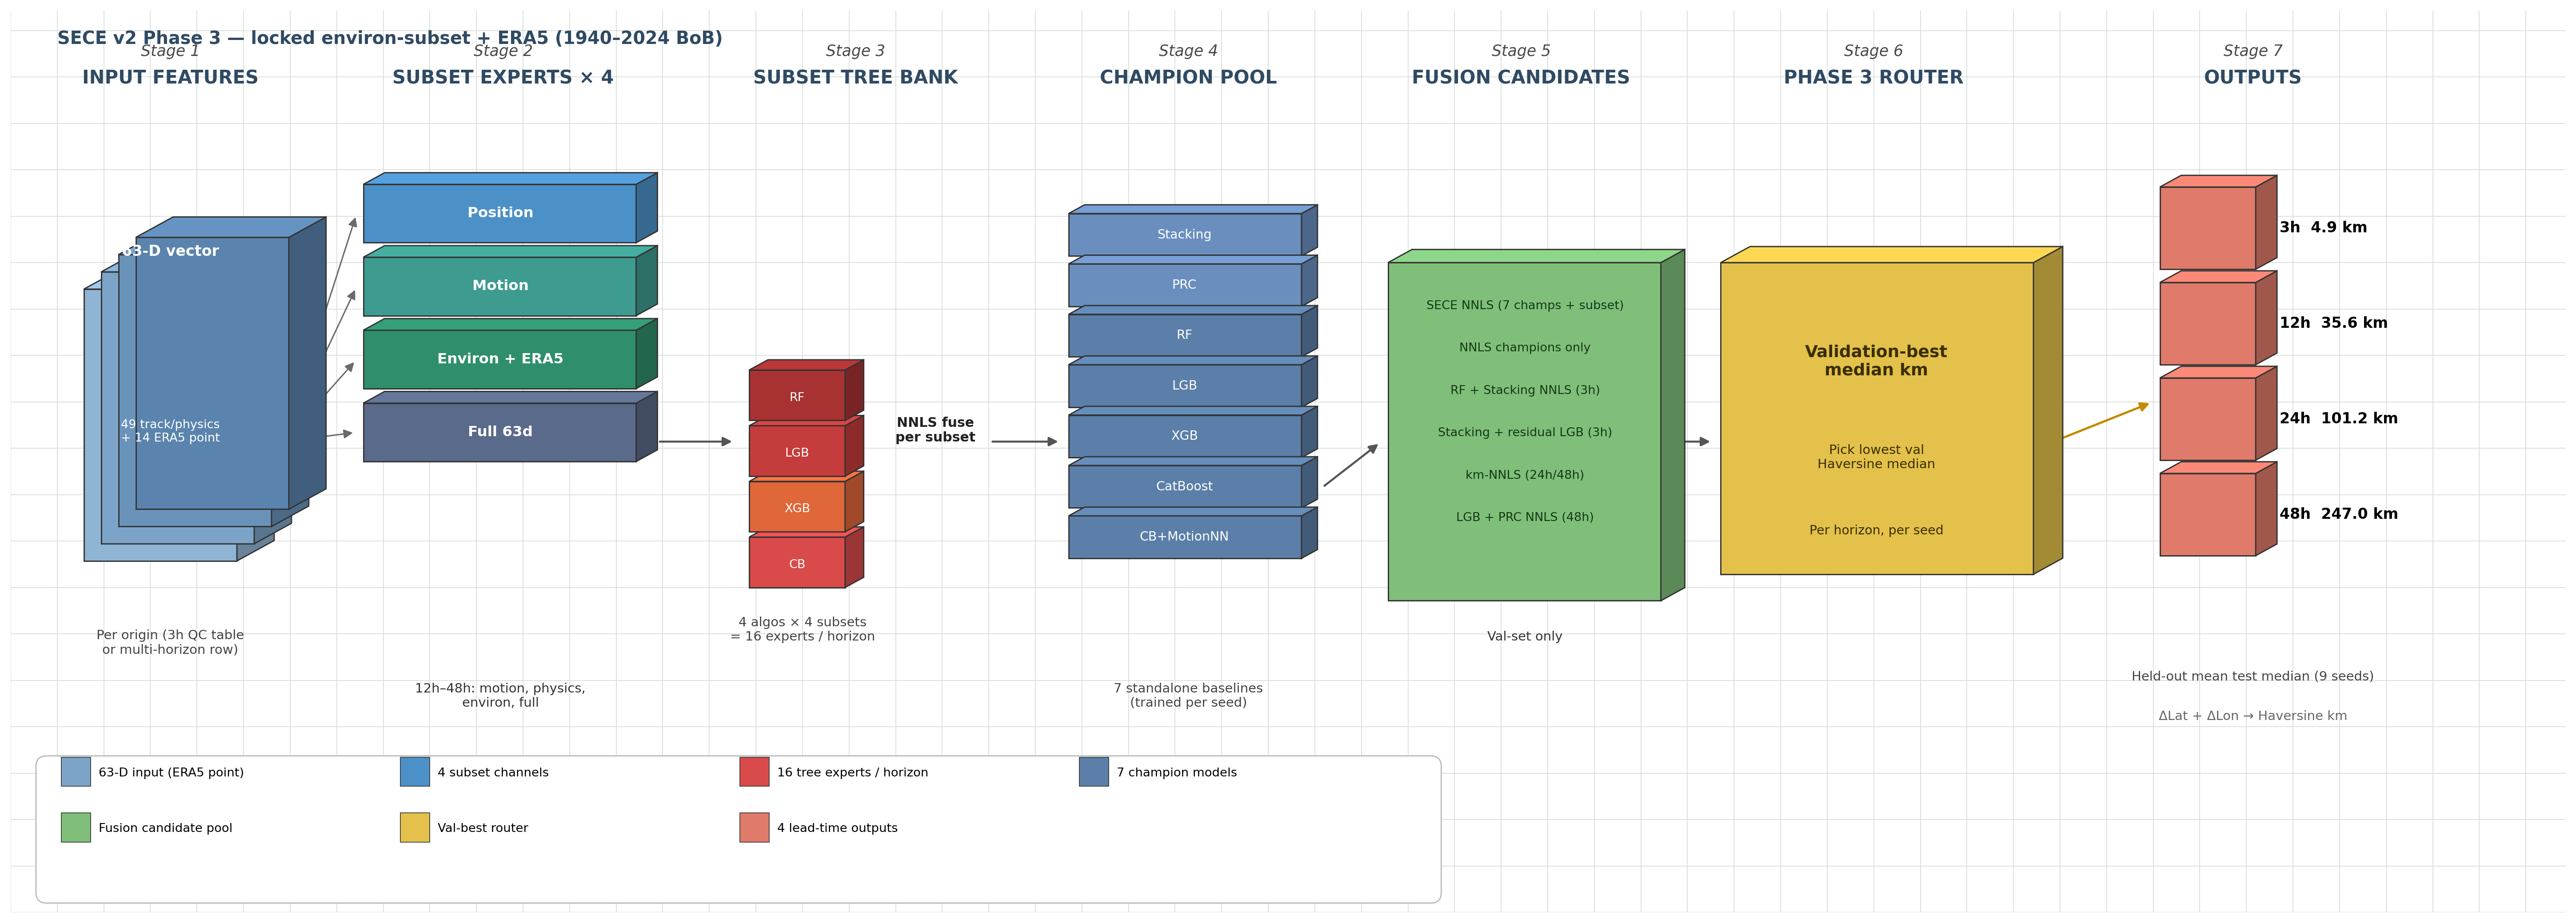
\includegraphics[width=\linewidth]{sece_phase3_architecture.png}
\caption{Locked \sece{} Phase~3 pipeline (63-D: 49 track/physics + 14 \era{} point features).}
\label{fig:arch}
\end{figure}

\begin{figure}[ht]
\centering

\includegraphics[width=\linewidth]{benchmark_3h_heldout.png}
\caption{Three-hour held-out benchmark: eight systems (Phase~3 environ subset).}
\label{fig:bench}
\end{figure}

\begin{figure}[ht]
\centering

\includegraphics[width=0.85\linewidth]{tsne_era5_63d.png}
\caption{t-SNE of 63-D training features ($n=10{,}000$ subsample).}
\label{fig:tsne}
\end{figure}

\begin{figure}[ht]
\centering

\includegraphics[width=0.9\linewidth]{case_study_laila_trajectories.png}
\caption{Laila (2010): IBTrACS vs.\ \sece{}, PRC, CB+MotionNN at 3, 12, 24\,h (held-out seed~0).}
\label{fig:laila}
\end{figure}

\begin{thebibliography}{30}
\bibitem{paul2010}B.~K. Paul, ``Human injuries caused by Bangladesh's cyclones Sidr and Aila,'' \textit{Nat. Hazards}, vol.~56, pp.~169--182, 2010.
\bibitem{mohapatra2015}M.~Mohapatra \textit{et al.}, ``Tropical cyclones over the North Indian Ocean,'' \textit{Mausam}, vol.~66, pp.~1--12, 2015.
\bibitem{demaria2013}M.~DeMaria \textit{et al.}, ``Tropical cyclone track and intensity forecasting,'' in \textit{Global Perspectives on Tropical Cyclones}, World Scientific, 2013, pp.~271--305.
\bibitem{goerss2000}J.~S. Goerss, ``Tropical cyclone track forecasts using an ensemble of dynamical models,'' \textit{Mon. Wea. Rev.}, vol.~128, pp.~1187--1193, 2000.
\bibitem{hersbach2020}H.~Hersbach \textit{et al.}, ``The ERA5 global reanalysis,'' \textit{Q. J. R. Meteorol. Soc.}, vol.~146, pp.~1999--2049, 2020.
\bibitem{knapp2010}K. R.~Knapp \textit{et al.}, ``The International Best Track Archive for Climate Stewardship (IBTrACS),'' \textit{Bull. Amer. Meteor. Soc.}, vol.~91, pp.~363--376, 2010.
\bibitem{walsh2015}K. J.~Walsh \textit{et al.}, ``Tropical cyclones and climate change,'' \textit{WIREs Clim. Change}, vol.~6, pp.~151--169, 2015.
\bibitem{neumann1972}C. J.~Neumann, ``An alternate to the HURRAN tropical cyclone forecast system,'' NOAA Tech. Memo., 1972.
\bibitem{kaplan2003}J.~Kaplan and M.~DeMaria, ``Large-scale characteristics of rapidly intensifying tropical cyclones,'' \textit{Wea. Forecasting}, vol.~18, pp.~1006--1015, 2003.
\bibitem{liu2020}Y.~Liu \textit{et al.}, ``Machine learning-based typhoon track prediction,'' \textit{IEEE Geosci. Remote Sens. Lett.}, vol.~17, pp.~1944--1948, 2020.
\bibitem{chen2020}S.~Chen \textit{et al.}, ``A deep learning model for tropical cyclone track forecast,'' \textit{Geophys. Res. Lett.}, vol.~47, e2020GL089597, 2020.
\bibitem{wu2018}L.~Wu \textit{et al.}, ``Global typhoon track forecast using a hybrid deep learning model,'' \textit{J. Meteor. Res.}, vol.~32, pp.~918--926, 2018.
\bibitem{grinsztajn2022}L.~Grinsztajn, E.~Oyallon, and G.~Varoquaux, ``Why do tree-based models still outperform deep learning on typical tabular data?'' \textit{Adv. Neural Inf. Process. Syst.}, vol.~35, 2022.
\bibitem{velden2006}C.~Velden \textit{et al.}, ``The Dvorak tropical cyclone intensity estimation technique,'' \textit{Bull. Amer. Meteor. Soc.}, vol.~87, pp.~1195--1210, 2006.
\bibitem{barnes2013}E. A.~Barnes, D.~H. W.~Fukomi, and T.~H.~Henderson, ``Storm track dynamics and climate change,'' \textit{J. Climate}, vol.~26, pp.~4993--5008, 2013.
\bibitem{prat2021}O.~Prat and C.~M.~Hennon, ``Tropical cyclone track forecasting using ERA5 data and machine learning,'' \textit{Wea. Forecasting}, vol.~36, pp.~123--138, 2021.
\bibitem{chan2005}J. C.~Chan, ``Interannual variations of tropical cyclone activity over the North Indian Ocean,'' \textit{Meteor. Atmos. Phys.}, vol.~89, pp.~143--152, 2005.
\bibitem{schreck2014}C. J.~Schreck \textit{et al.}, ``A long-term high-resolution dataset of the North Atlantic best track and climate,'' \textit{J. Climate}, vol.~27, pp.~3698--3713, 2014.
\bibitem{gneiting2014}T.~Gneiting and M.~Katzfuss, ``Probabilistic forecasting,'' \textit{Annu. Rev. Stat. Appl.}, vol.~1, pp.~125--151, 2014.
\bibitem{cawley2010}G.~C. Cawley and N.~L.~C. Talbot, ``On over-fitting in model selection,'' \textit{J. Mach. Learn. Res.}, vol.~11, pp.~2079--2107, 2010.
\bibitem{kossin2013}J. P.~Kossin, ``Trends in western North Pacific tropical cyclone intensity,'' \textit{Eos Trans. AGU}, vol.~94, pp.~233--241, 2013.
\bibitem{ritchie2014}E.~Ritchie and J.~Elsberry, ``Tropical cyclone track predictability,'' \textit{Meteor. Monogr.}, vol.~56, pp.~1--24, 2014.
\bibitem{probst2019}P.~Probst, A.~L.~Boulesteix, and A.~Bischl, ``Tunability of ML hyperparameters,'' \textit{J. Mach. Learn. Res.}, vol.~20, pp.~1--32, 2019.
\bibitem{lee2021}C.~Lee \textit{et al.}, ``Ensemble deep learning for tropical cyclone track prediction,'' \textit{Remote Sens.}, vol.~13, Art.~no.~4521, 2021.
\bibitem{sampson2018}C.~Sampson \textit{et al.}, ``Objective guidance for tropical cyclone forecasting,'' \textit{Wea. Forecasting}, vol.~33, pp.~683--698, 2018.
\bibitem{berg2013}E.~Berg \textit{et al.}, ``Tropical cyclone wind speed estimation from satellite imagery,'' \textit{Wea. Forecasting}, vol.~28, pp.~783--794, 2013.
\bibitem{moller2018}A.~M\"oller \textit{et al.}, ``Probabilistic forecasts for tropical cyclone tracks,'' \textit{Wea. Forecasting}, vol.~33, pp.~79--92, 2018.
\bibitem{emanuel2005}K.~Emanuel, ``Increasing destructiveness of tropical cyclones,'' \textit{Nature}, vol.~436, pp.~686--688, 2005.
\bibitem{reichstein2019}M.~Reichstein \textit{et al.}, ``Deep learning and process understanding for data-driven Earth system science,'' \textit{Nature}, vol.~566, pp.~195--204, 2019.
\bibitem{holland1983}G.~J. Holland, ``Tropical cyclone motion: Environmental interaction plus a beta effect,'' \textit{J. Atmos. Sci.}, vol.~40, pp.~328--342, 1983.
\end{thebibliography}

\end{document}
